\chapter{Analyse de Fourier des systèmes à temps discret}
Dans le cas d'un signal périodique, la série de Fourier était utilisée
\begin{equation}
x(t) = \sum_{k=-\infty}^\infty a_ke^{jk\omega_0t}\qquad a_k = \frac{1}{T}\int_T
x(t)e^{-jk\omega_0t}
\end{equation}
où l'on peut voir $a_k$ comme le coefficient de pondération de chaque exponentielle 
complexe. Dans le cas ou les signaux n'étaient pas périodiques, la \textit{transformée 
de Fourier} (et inverse) a (ont) été définie(s)
\begin{equation}
X(j\omega) = \int_{-\infty}^\infty x(t)e^{-j\omega t}\ dt,\qquad x(t)=\frac{1}{2\pi}
\int_{-\infty}^\infty X(j\omega)e^{j\omega t}\ d\omega
\end{equation}
Le \textit{théorème de convolution} peut permettre un traitement plus aisé de la 
convolution
\begin{equation}
y(t) = x(t)*h(t)\qquad \ft\qquad Y(j\omega) = X(j\omega)H(j\omega)
\end{equation}

\section{Réponse à une exponentielle complexe}
Considérons l'entrée suivante
\begin{equation}
x(n) = z^n,\quad z=e^{j\omega_0}\qquad\Rightarrow\qquad x(n) = e^{j\omega_0n}
\end{equation}
où $-\infty<n<\infty$. Le signal de sortie est donnée en effectuant la convolution
\begin{equation}
\begin{array}{ll}
y(n) &= \sum_{k=-\infty}^\infty h(k)x(n-k) = \sum_{k=-\infty}^\infty h(k)z^{n-k} = z^n 
\underbrace{\sum_{k=-\infty}^\infty h(k)z^{-k}}_{H(z) \in \mathbb{C}}\\
&= H(z)z^n
\end{array}
\end{equation}
En effet, la dernière somme peut être vue comme une constante complexe (dépendant de $z$ 
et du SLP). Cette sortie  n'est que la fonction d'entrée multipliée par quelque chose : 
$z^n,z\in\mathbb{C}$ est une \textit{fonction propre} de tout SLP discret.\\
Si par hasard le signal d'entrée peut se mettre sous la forme d'une somme d'exponentielle 
complexe (fonction propre) multipliée par un scalaire
\begin{equation}
x(n) = \sum_p a_pz_p^n
\end{equation}
La réponse s'obtient par simple application de la linéarité
\begin{equation}
y(n) = \sum_p a_pH(z_p)z_p^n
\end{equation}
Ceci justifie l'analyse de Fourier pour les systèmes discrets.

\section{Série de Fourier discrète}
Il est possible de développer en série de Fourier un signal périodique (période $T_0$) 
à T\textbf{C} $x(t)$ 
\begin{equation}
x(t) = \sum_{k=-\infty}^\infty a_k e^{jk\frac{2\pi}{T_0}t}
\end{equation}
Il est dès lors tentant de vouloir faire de même pour un signal à T\textbf{D} périodique, 
de période $N$ ($x(n)=x(n+N)$) comme une combili d'exponentielle discrète de période $N$.\\
Nous avions vu qu'il n'existe que $N$ exponentielles discrètes distinctes de période $N$. 
C'est le cas ssi
\begin{equation}
\omega_0 = m\dfrac{2\pi}{N}\qquad m\in\mathbb{Z}
\end{equation}
La sommation est ainsi limitée à ces $N$ termes
\begin{equation}
x(n) = \sum_{k=0}^{N-1} a_ke^{jk\frac{2\pi}{N}n}\qquad n=0,1,\dots,N-1
\label{eq:syst}
\end{equation}
Il faut ainsi résoudre un système de $N$ équations à $N$ inconnues pour déterminer les $a_k$ 
d'une série $x(n)$ donnée :
\begin{equation}
\left\{\begin{array}{ll}
x(0) &= \sum_{k=0}^{N-1} a_k\\
x(1) &= \sum_{k=0}^{N-1} a_ke^{jk\frac{2\pi}{N}}\\
\vdots\\
x(N-1) &= \sum_{k=0}^{N-1} a_ke^{jk\frac{2\pi}{N}(N-1)}
\end{array}\right.
\end{equation}

	\exemple{Déterminons la série de Fourier $x(n) = \sum_{k=0}^{N-1} a_ke^{jk\frac{2
	\pi}{N}n}\qquad n=0,1,\dots,N-1$ du signal ci-dessous (1,0,2,-1,\dots).
	\begin{center}
	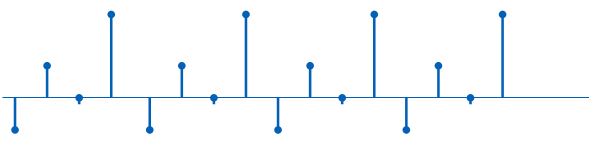
\includegraphics[scale=0.45]{ch3/image1.png}
	\captionof{figure}{ }
	\end{center}
	La série doit vérifier les points donnés, c'est-à-dire que le système ci-dessous 
	doit être satisfait.
	\begin{equation}
	\left\{\begin{array}{llll}
	x(0) &=1 &= \sum_{k=0}^{4-1} a_ke^{j2\pi k0/4} &= a_0+a_1+a_2+a_3\\
	x(1) &=0 &= \sum_{k=0}^{4-1} a_ke^{j2\pi k1/4} &= a_0+ja_1-a_2-ja_3\\
	x(2) &=2 &= \sum_{k=0}^{4-1} a_ke^{j2\pi k2/4} &= a_0-a_1+a_2-a_3\\
	x(3) &=-1 &= \sum_{k=0}^{4-1} a_ke^{j2\pi k3/4} &= a_0-ja_1-a_2+ja_3		
	\end{array}\right.\quad\Leftrightarrow\quad\left\{\begin{array}{ll}
	a_0 &= 1/2\\
	a_1 &= -\frac{1+j}{4}\\
	a_2 &= -1\\
	a_3 &= -\frac{1-j}{4}
	\end{array}\right.
	\end{equation}}

\newpage
Cette représentation n'est valable que si l'on peut exprimer les $a_k$ à partir de 
$x(n)$ : il faut résoudre le système de $N$ équations à $N$ inconnues \autoref{eq:syst}. 
Il faut pour cela calculer
\begin{equation}
\begin{array}{ll}
\displaystyle\sum_{n=0}^{N-1} x(n)e^{-jm\frac{2\pi}{N}n} &= \displaystyle\sum_{n=0}^{N-1}
\sum_{k=0}^{N-1} a_k e^{j(k-m)\frac{2\pi}{N}n}\\
&=\displaystyle \sum_{k=0}^{N-1} a_k \sum_{n=0}^{N-1} e^{j(k-m)\frac{2\pi}{N}n}
\end{array}
\end{equation}
La dernière somme peut être écrite
\begin{equation}
S = \sum_{n=0}^{N-1}e^{-j(k-m)\frac{2\pi}{N}n}  = \sum_{n=0}^{N-1} \alpha^n
\end{equation}
où $\displaystyle \alpha = e^{-j(k-m)\frac{2\pi}{N}}$. Il s'agit de la série géométrique
\begin{equation}
S = \left\{\begin{array}{ll}
N & \text{ si } \alpha = 1\quad \text{c-à-d si } k-m=0,\pm N,\pm 2N,\dots\\
\dfrac{1-\alpha^N}{1-\alpha} & \text{ si } \alpha \neq 1\quad \text{car } 
\alpha^N = 1
\end{array}\right.
\end{equation}
ou encore
\begin{equation}
S=\left\{\begin{array}{ll}
N &\text{ si } k-m = 0,\pm N, \pm 2N,\dots\\
0 &\text{ sinon}
\end{array}\right.
\end{equation}
Si $m\in[0;N-1]$, $S$ ne sera non nulle que pour $k=m$ et donc, en isolant
\begin{equation}
a_m = \frac{1}{N}\sum_{n=0}^{N-1} x(n)e^{-jm\frac{2\pi}{N}n}\qquad m=0,\dots,N-1
\label{eq:nouv}
\end{equation}
soit l'expression des coefficients de la série de Fourier discrète.


	\exemple{Reconsidérons le précédent exemple. Nous devrions retrouver les mêmes 
	coefficients à partir de \autoref{eq:nouv}. Nous avons ici
	\begin{equation}
	a_m = \frac{1}{4}\sum_{n=0}^{4-1} x(n)e^{-jm\frac{2\pi}{N}n} = \frac{1}{4}
	\left(1+2e^{-jm\pi}-e^{-jm3\pi/2}\right)
	\end{equation}
	On retrouve bien les mêmes coefficients.
	\begin{equation}
	\left\{\begin{array}{ll}
	a_0 &= 1/2\\
	a_1 &= -\frac{1+j}{4}\\
	a_2 &= -1\\
	a_" &= -\frac{1-j}{4}
	\end{array}\right.
	\end{equation}}\ \\
	
	
	\exemple{Pour le fun, calculons les coefficients de la série de Fourier de 
	$x(n) = \sin\left(\dfrac{2\pi}{N}n\right)$. On peut également écrire
	\begin{equation}
	x(n) = \dfrac{e^{j\frac{2\pi}{N}n}-e^{-j\frac{2\pi}{N}n}}{2j}
	\end{equation}
	La série de Fourier ayant la forme $x(n) = \sum_{k=0}^{N-1} a_ke^{j2\pi kn/N}$, 
	on en déduit directement les coefficients par identification
	\begin{equation}
	a_1 = \frac{1}{2j},\qquad a_{-1} = -\frac{1}{2j},\qquad a_x=0\ \text{sinon}.
	\end{equation}}


\newpage
Ceci montre que $x(n)$ est intégralement (pfpfpf) défini par $N$ paramètres\footnote{
Les $N$ valeurs du signal sur une période.} ; la série de Fourier discrète transforme 
ces $N$ paramètres en $N$ paramètres $a_k$. Nous utiliserons les notations suivantes 
(déplacement du facteur $1/N$) :
\begin{equation}
X(k) = \sum_{n=0}^{N-1} x(n)e^{-j\frac{2\pi}{N}nk},\qquad x(n) =\frac{1}{N}\sum_{
k=0}^{N-1} X(k)e^{j\frac{2\pi}{N}kn}
\end{equation}
où $X(k)$ ($=X(k+N)$) est la \textit{transformée de Fourier discrète} (DFT) de $x(n)$.\\
La linéarité appliquée en début de chapitre pour la sortie d'un SLP s'applique également 
ici de sorte que la sortie sera donnée par
\begin{equation}
y(n) = \frac{1}{N}\sum_{k=0}^{N-1} X(k)H\left(e^{j\frac{2\pi}{N}k}\right)
e^{j\frac{2\pi}{N}kn}\qquad \text{ où }\quad H\left(e^{j\frac{2\pi}{N}k}\right) = 
\sum_{n=-\infty}^\infty h(n)e^{-j\frac{2\pi}{N}kn}
\end{equation}
Il s'agit d'une convolution où $x$ est remplacé par sa série de Fourier.
	
\section{Réponse en fréquence d'un système discret}
En considérant comme signal d'entrée discret $x(n) = e^{j\omega n}$ (exponentielle unitaire), 
celle-ci étant fonction propre notre sortie sera
\begin{equation}
y(n) = H\left(e^{j\omega }\right)e^{j\omega n}
\end{equation}
où $\displaystyle H\left(e^{j\omega }\right) = \sum_{k=-\infty}^\infty h(k)e^{-j
\omega k}$ est la réponse en fréquence du système\footnote{On met une grandeur unitaire 
en entrée et on fait varier $\omega$ pour voir comment déduire en fréquence.}. L'idée 
est que $H$ ne soit évalué que sur le cercle unitaire. Il s'agit d'une constante complexe 
pour $\omega$ fixé
\begin{equation}
H\left(e^{j\omega }\right) = \left|H\left(e^{j\omega }\right)\right|e^{j\text{arg} 
H\left(e^{j\omega }\right)}
\end{equation}
Dès lors, pour un signal d'entrée réel du type $x(n) = A\cos(\omega_0n+\varphi)$, la 
sortie vaut (superposition)
\begin{equation}
y(n) = A \left|H\left(e^{j\omega_0 }\right)\right|\cos\left(\omega_0n+\varphi+\text{arg} 
H\left(e^{j\omega_0}\right)\right)
\end{equation}
On peut considérer $H\left(e^{j\omega}\right)$ comme le développement de la fonction 
périodique $H$ en série de Fourier (où $\omega$ est continu). Dès lors, on peut exprimer 
les échantillons $h(k)$ par la formule classique de calcul des coefficients d'une série 
de Fourier
\begin{equation}
h(k) = \frac{1}{2\pi}\int_{-\pi}^\pi H\left(e^{j\omega }\right)e^{j\omega k}\ d\omega
\end{equation}
exprimant la réponse impulsionnelle en fonction de la réponse fréquentielle.


\exemple{Slide T32/34}

\newpage
\section{Transformée de Fourier d'un signal discret}
Les deux relations
\begin{equation}
H(e^{j\omega}) = \sum_{k=-\infty}^\infty h(k)e^{-j\omega k},\qquad\qquad h(k) = \dfrac{1}{2\pi}
\int_{-\pi}^\pi H(e^{j\omega}) e^{j\omega k}\ d\omega
\end{equation}
étaient utilisées pour calculer le spectre de la réponse impulsionnelle et son 
retour au domaine temporel ne se limite \textbf{pas} à elles : n'importe quel signal discret 
peut être transformé, même les \textbf{apériodiques} (différence avec la série de Fourier qui 
est nécessairement périodique).\\
La \textit{transformée de Fourier (et inverse) d'un signal apériodique} est définie par
\begin{equation}
X(e^{j\omega}) = \sum_{n=-\infty}^\infty x(n)e^{-j\omega n},\qquad\qquad x(n) = \dfrac{1}{2\pi}
\int_{-\pi}^\pi X(e^{j\omega}) e^{j\omega n}\ d\omega
\end{equation}
La limitation sur $(-\pi,\pi)$ permet de considérer toutes les exponentielles complexes 
distinctes, évitant ainsi les répétitions. \\
Étudions la convergence de $X(e^{j\omega})$. Pour converger, $x(n)$ doit être absolument sommable
\begin{equation}
\sum_{n=-\infty}^\infty |x(n)|<\infty
\end{equation}
Si ceci est vrai, cela implique la convergence uniforme vers une fonction continue de $\omega$ : 
la réponse en fréquence d'un système stable converge toujours.  Une autre manière de vérifier la 
convergence est de vérifier que la transformée est de carré sommable (énergie finie)
\begin{equation}
\sum_{n=-\infty}^\infty |x(n)|^2<\infty
\end{equation}
Notons que toute fonction de carré sommable est forcément absolument sommable.

	\subsection{Propriétés de la transformée de Fourier}
	Bien évidemment, cette transformée est linéaire (étant elle même une combili, ceci peut 
	paraître logique). Différentes symétries sont proposées au slide T37, ceci ne sera pas 
	revu ici.
	
		\subsubsection{Glissement}
		\begin{equation}
		\begin{array}{ll}
		x(n-n_0) &\Leftrightarrow e^{-j\omega n_0}X(e^{j\omega})\\
		e^{j\omega_0n}x(n) &\Leftrightarrow X\left(e^{j(\omega-\omega_0)}\right)
		\end{array}		
		\end{equation}


		\subsubsection{Parseval}
		\begin{equation}
		\sum_{n=-\infty}^\infty |x(n)|^2 = \dfrac{1}{2\pi}\int_{-\pi}^\pi \left|X(e^{j\omega})\right|^2\ 
		d\omega
		\end{equation}
		Ceci montre que les énergie dans le domaine temporel correspondent aux énergie dans le 
		domaine fréquentiel. 
		
		\subsubsection{Convolution}
		Considérons notre convolution fétiche : $y(n) = h(n)*x(n) = \DS \sum_{k=-\infty}^\infty 
		h(n-k)x(k)$. Calculons le spectre de $y(n)$
		\begin{equation}
		\begin{array}{ll}
		Y(e^{j\omega}) &= \DS \sum_{n=-\infty}^\infty y(n)e^{-j\omega n} = \sum_{n=-\infty}^\infty
		\sum_{k=-\infty}^\infty h(n-k)x(k)e^{-j\omega n}\\
		&= \DS\sum_{k=-\infty}^\infty x(k) \sum_{n=-\infty}^\infty h(n-k)e^{-j\omega n}\\
		&= \DS \sum_{k=-\infty}^\infty x(k)e^{-j\omega k} \sum_{n=-\infty}^\infty h(n-k)
		e^{-j\omega(n-k)} = X(e^{j\omega})H(e^{j\omega})
		\end{array}
		\end{equation}
		La dernière étape fait apparaître la définition des spectres $X$ et $H$. Le résultat 
		n'est qu'une simple multiplication dans le domaine fréquentiel.
		
		\subsubsection{Modulation}
		Soit $y(n) = x_1(n)x_2(n)$. En calculant le spectre\footnote{La démonstration se trouve dans le cours d'analyse complexe}
		\begin{equation}
		\begin{array}{ll}
		Y(e^{j\omega}) &= \DS \dfrac{1}{2\pi}\int_{-\pi}^\pi X_1(e^{j\theta})X_2(e^{j(\omega-\theta)})\ 
		d\theta\\
		&= \DS \dfrac{1}{2\pi}X_1(e^{j\omega}) \otimes X_2(e^{j\omega})
		\end{array}
		\end{equation}
		où $\otimes$ est la convolution périodique des deux spectres.


\section{Transformée de Fourier des signaux périodiques}
Regardons ce que donne cette transformée pour un signal périodique ("\textit{qui peut le plus peut 
le moins" }). Soit $x_1(n)$ un signal \textbf{a}périodique, de transformée de Fourier $X_1(e^{j\omega})$.
Construisons un signal périodique $x(n)$ de période $N$ 
\begin{equation}
x(n) = \sum_{r=-\infty}^{\infty} x_1(n+rN)
\end{equation}
Il existe d'autres façon de construire un tel signal. Calculons les coefficients $X_d(k)$ de la 
série (car périodique) de Fourier (discrète) de $x(n)$ (en substituant l'expression de $x(n)$) :
\begin{equation}
\begin{array}{ll}
X_d(k) &=\DS \sum_{n=0}^{N-1} x(n) e^{-j\frac{2\pi}{N}nk} = \sum_{n=0}^{N-1}\sum_{r=-\infty}^{\infty} x_1(n+rN)
 e^{-j\frac{2\pi}{N}nk}\\
 &=\DS \sum_{n=0}^{N-1}\sum_{r=-\infty}^{\infty} x_1(n+rN) e^{-j\frac{2\pi}{N}(n+rN)k}
 \end{array}
\end{equation}
En décomposant l'expression ci-dessous, on retrouve l'exponentielle de départ avec en plus un
nombre fixe de fois $2\pi$ ($e^{jx}$ est périodique, de période $2\pi : e^{j2\pi}=1$, cela ne 
change donc rien) :
\begin{equation}
X_d(k) = \sum_{m=-\infty}^\infty x_1(m)e^{-j\frac{2\pi}{N}mk} = X_1(e^{j\frac{2\pi}{N}k})
\end{equation}
On passe ainsi en revue toutes les valeurs de $x_1(n)$ avec une exponentielle complexe associée : 
ces coefficients sont les échantillons de $X_1(e^{j\omega})$ prélevés à intervalle $2\pi/N$. Le 
spectre est quelque chose de connu : $X_d(k)$ échantillons à intervalles réguliers, directement 
relié à la transformée de Fourier du signal qui n'était \textbf{pas} périodique.\\

Prenons la transformée de Fourier du signal périodique $x(n)$ en appliquant la propriété du 
glissement ($\DS x(n) = \sum_{r=-\infty}^\infty x_1(n+rN)$)
\begin{equation}
X(e^{j\omega}) = \sum_{r=-\infty}^\infty X_1(e^{j\omega})e^{j\omega rN} = X_1(e^{j\omega})\sum_{
r=-\infty}^\infty e^{j\omega rN}
\end{equation}
Le spectre du signal périodique est directement lié au spectre du signal apériodique. On établit que
\begin{equation}
\sum_{r=-\infty}^\infty e^{j\omega rN} = \dfrac{2\pi}{N}\sum_{k=-\infty}^\infty \delta\left(
\omega-k\dfrac{2\pi}{N}\right)
\end{equation}
Ce qui n'est rien d'autre qu'un train d'impulsions.\\

Cet "établi" peut sembler suspect. Comme nous sommes à l'ULB (libre examen patatipatata), montrons 
en effet que 
\begin{equation}
\Delta_T(t) := \sum_{k=-\infty}^\infty \delta(t-kT)
\end{equation}
Comme celui-ci est périodique ($\Delta_T(t+T)=\Delta_T(t)$), on peut calculer sa série de Fourier 
(définie ici en discret pour la somme, mais le domaine est bien \textbf{continu} ! (On l'a déjà 
fait en discret dans le passé). 
\begin{equation}
\Delta_T(t) = \sum_{n=-\infty}^\infty c_ne^{i2\pi nt/T}
\end{equation}
Calculons donc ses coefficients
\begin{equation}
\begin{split}
c_n &=  \frac{1}{T}\int_{t_0}^{t_0+T} \Delta_T(t)e^{-i2\pi nt/T}\ dt\qquad (-\infty < t_0<+\infty)\\
&= \frac{1}{T}\int_{-T/2}^{T/2} \Delta_T(t)e^{-i2\pi nt/T}\ dt \\
&= \frac{1}{T}\int_{-T/2}^{T/2} \delta(t) e^{-i2\pi nt/T}\ dt \\
&= \frac{1}{T} e^{-i2\pi n0/T}\\
&= \frac{1}{T}
\end{split}
\end{equation}
En effet, une période correspond à l'intervalle $[-T/2,T/2]$. Sur cette intervalle on retrouve une 
seule impulsion (en zéro), les autre sont en dehors d'où le $\delta(t)$. On a donc
\begin{equation}
\Delta_T(t) = \dfrac{1}{T}\sum_{n=-\infty}^\infty e^{i2\pi nt/T}
\end{equation}
En effectuant le changement de variable $t\rightarrow\omega$ et $T\rightarrow 2\pi/N$,  on retrouve
\begin{equation}
\sum_{r=-\infty}^\infty e^{j\omega rN} = \dfrac{2\pi}{N}\sum_{k=-\infty}^\infty \delta\left(\omega-k\frac{2\pi}{N}
\right)
\end{equation}

Revenons à notre somme de train d'impulsion. Comme le signal n'est non-nul que lorsque 
$\omega = k\frac{2\pi}{N}$ :
\begin{equation}
\begin{array}{ll}
X(e^{j\omega}) &= \DS X_1(e^{j\omega})\dfrac{2\pi}{N}\sum_{k=-\infty}^\infty \delta\left(
\omega-k\dfrac{2\pi}{N}\right)\\
&=\DS \dfrac{2\pi}{N}\sum_{k=-\infty}^\infty X_1\left(e^{j\frac{2\pi}{N}k}\right)\delta\left(
\omega-k\dfrac{2\pi}{N}\right)\\
&=\DS \sum_{k=-\infty}^\infty \frac{2\pi}{N} X_d(k)\delta\left(\omega-k\dfrac{2\pi}{N}\right)\\
\end{array}
\end{equation}
Il s'agit de la transformée de Fourier d'un signal périodique en fonction de son développement 
en série de Fourier discrète sur le spectre du signal apériodique : on retrouve "seulement" les 
coefficnets de la série de Fourier. Le signal périodique $x(n)$ possède une série de raie espacée de $2\pi/N$.\\

Un exemple et un résumé du chapitre sont donnés au slide T45 et T46.





